\chapter{Análisis del problema}

\section{Elección de un sistema operativo}

\subsection{¿SO de propósito general o sistema operativo de tiempo real?}

El principal rol del sistema operativo es controlar los recursos del sistema para suplir las demandas de las aplicaciones que trabajan sobre él. Todos los SOs, independientemente de si son de propósito general o de tiempo real, tienen elementos esenciales tales como la planificación de procesos, control de memoria, relojes, entrada/salida, etcétera. 

Si bien comparten dichos elementos esenciales, los RTOS están diseñados con la filosofía de que sus tiempos de espera, procesamiento y respuesta son más importantes que su rendimiento promedio. Los RTOS se utilizan en los casos en los procesos deban estar planificados en el tiempo, garantizando que se cumplan los requerimientos temporales para dichos procesos. 

En el caso de este proyecto, se necesita que el SO a escoger tenga baja latencia, que pueda asegurar que las tareas que lo requieran terminarán en el tiempo determinado, así como permitir que las tareas críticas y no críticas coexistan en el sistema. También es muy importante que dicho SO tenga un sistema de asignación de prioridades que permita al programador establecer cuáles son las tareas y procesos más importantes para su proyecto y darles esa importancia en la ejecución.

\subsection{¿RTOS comercial o de código abierto?}

Si bien los RTOS comerciales ofrecen una mayor variedad de funciones para el programador, sus precios suelen ser demasiado elevados para poder escogerlos en un proyecto como este. Por ejemplo, en el caso de VxWorks, el RTOS propietario líder en el sector, de la empresa Wind River, el precio del SO comienza en los 18500\$ per seat (por usuario que trabaja con el sistema). Obviamente esto es algo prohibitivo para nuestro presupuesto, pero en el caso de una ECU que se implemente en vehículos sería la mejor opción.\newline

Pero no todos los RTOS son comerciales, sino que existen multitud de ellos que son de código abierto. A continuación se expone una tabla con las principales características de algunos de los RTOS \textit{open source} más importantes:

\begin{table}[H]
    \resizebox{\columnwidth}{!}{%
    \begin{tabular}{|l|l|l|l|}
    \hline
    \rowcolor[HTML]{CBCEFB} 
    \textbf{Nombre} &
      \textbf{Aplicación principal} &
      \textbf{\begin{tabular}[c]{@{}l@{}}Facilidad de \\ programación\end{tabular}} &
      \textbf{\begin{tabular}[c]{@{}l@{}}Eficiencia en \\ ECU\end{tabular}} \\ \hline
    \textbf{RIOT}        & \begin{tabular}[c]{@{}l@{}}Orientado a dispositivos de\\  Internet de las Cosas (IoT)\end{tabular} & Media   & Media \\ \hline
    \textbf{Nano-RK}     & \begin{tabular}[c]{@{}l@{}}Sistemas embebidos en\\ tiempo real\end{tabular}                        & Difícil & Alta  \\ \hline
    \textbf{FreeRTOS}    & \begin{tabular}[c]{@{}l@{}}Sistema operativo de tiempo\\  real de código abierto\end{tabular}      & Media   & Media \\ \hline
    \textbf{ARM mbed OS} & Plataforma de desarrollo para IoT                                                                  & Fácil   & Alta  \\ \hline
    \textbf{Raspbian}    & \begin{tabular}[c]{@{}l@{}}Sistema operativo general\\  para Raspberry Pi\end{tabular}             & Fácil   & Baja  \\ \hline
    \textbf{DuinOS}      & \begin{tabular}[c]{@{}l@{}}RTOS diseñado específicamente\\  para Arduino\end{tabular}              & Fácil   & Baja  \\ \hline
    \textbf{mipOS}       & \begin{tabular}[c]{@{}l@{}}RTOS de código abierto para\\  sistemas embebidos\end{tabular}          & Media   & Baja  \\ \hline
    \end{tabular}%
    }
    \end{table}

Para escoger, comenzamos por descartar todos aquellos sistemas operativos que se utilicen para IoT, pues normalmente las restricciones de tiempo en esos sistemas son mucho más suaves. Si hacemos un balance entre la facilidad de programación y la eficiencia, pues el tiempo de desarrollo es bastante limitado y diseñar un programa en los sistemas más difíciles puede requerir demasiado tiempo, encontramos que la mejor alternativa es FreeRTOS. 

\subsubsection*{FreeRTOS}

FreeRTOS es uno de los RTOS más utilizados para microcontroladores y pequeños microprocesadores, con soporte para una gran variedad de placas. Tiene una proyección \textbf{LTS} (\textit{Long Term Support}), lo que garantiza que el proyecto podrá seguir teniendo soporte a largo plazo. Una de sus grandes ventajas es la gran cantidad de librerías modulares, así como también el enfoque del kernel para ahorrar energía y no ser demasiado pesado. 

Por todas estas razones, FreeRTOS es la elección perfecta para un proyecto con estas características. 

\section{Elección de la placa}
\subsection{Requisitos}
A la hora de escoger la placa existen varios requisitos básicos debe cumplir, nombrados a continuación: 

\subsubsection*{Soporte de FreeRTOS}

El primer requisito es que FreeRTOS soporte la placa que vayamos a escoger. Por suerte, este SO está ampliamente compatibilizado y existen multitud de placas disponibles[25]. Entre ellos están las placas de Altera, Infineon, Raspberry Pi, e incluso los usuarios han desarrollado FreeRTOS compatible con Arduino.

\subsubsection*{Precio}

Si bien algunas de las placas anteriormente nombradas son objetivamente mejores, el presupuesto es limitado y requerimos de una placa que, como precio máximo, cueste 50\$. Con esto descartamos las placas de Altera e Infineon, así como una gran multitud de marcas que están orientadas a proyectos de ámbito profesional. 

\subsubsection*{Rendimiento y frecuencia de reloj}

Al ser un proyecto con RTOS, se necesita que la placa tenga una frecuencia de reloj que permita realizar las funciones más importantes en un periodo corto, incluso en el peor caso. Para comenzar con la estimación, debemos destacar aquellas funciones del sistema que tengan el plazo más restrictivo. 

En el caso de la comprobación de la temperatura de batería y motor, debe de medirse dicha temperatura cada muy poco tiempo, asegurando así que el sistema no se esté sobrecalentando y pueda provocar un problema. 

Para realizar dichas mediciones, tendremos en cuenta dos funciones necesarias. 

\begin{enumerate}
    \item Inicio del sensor: Los sensores que se utilizan para medir temperaturas tienen un tiempo mínimo de 1s para conseguir la temperatura correcta, por lo que se iniciará y, un segundo después, se avisará a la segunda función.
    \item Comprobación de la temperatura: La ECU leerá los valores que le ha mandado el sensor en el último segundo y, mediante una ecuación, hallará el valor en grados celsius correspondiente. Tras hacer esto, comparará el valor con el límite superior que definen el intervalo de temperaturas correctas y, si no está dentro de dichos valores, enviará una señal a otra función que mostrará el aviso de temperatura por pantalla. 
\end{enumerate}

La segunda función es la que nos marcará el mínimo valor necesario de frecuencia de reloj para que el sistema pueda funcionar correctamente, realizando mediciones cada 100 ms. Para poder hallar entonces cuál es ese valor, programamos con pseudocódigo de manera básica una función que realice el proceso:


Se ha tomado como referencia un sensor LM35 cuya ecuación para hallar la temperatura es la siguiente: 

\begin{verbatim}
    Temperatura = Valor * 5 * 100 /1024
\end{verbatim}


\begin{verbatim}
    subproceso funcion temperatura_bateria
        tempB <- leer(sensor)
        temB <- (tempB * 5 * 100) / 1024
        si tempB > 45
            entonces temp_error = 1
        fin si
    fin funcion
\end{verbatim}

Teniendo ya este pseudocódigo, podemos estimar de manera aproximada la cantidad de ciclos y las instrucciones necesarias para llevar a cabo esta función, por lo que necesitamos convertir este código a ensamblador: 

\begin{verbatim}
    LDR rdi, #SENSOR 
    MUL $0.48828125, rdi
    CMP rdi, $45
    JA .L1
    MOV $1, rsi

    .L1
\end{verbatim}

Por motivos de eficiencia se ha reducido la operación de la fórmula al mínimo posible. 

Teniendo en cuenta que la operación que mayor número de cicos necesita, que es LOAD, con cinco ciclos, vamos a aproximar el número de ciclos del resto de instrucciones a 5 para poseer mayor margen en el cálculo a la hora de escoger la frecuencia de reloj necesaria.

Por tanto, nuestro programa tardará como mínimo 5 * 5 = 25 ciclos de reloj.

Ahora, teniendo en cuenta lo aprendido en la asignatura de Arquitectura de Computadores, vamos a hallar la frecuencia de reloj mínima para que el sistema pueda realizar este proceso en el tiempo determinado de 10ms. Utilizaremos la siguiente fórmula: 

\begin{align*}
    T_{CPU} = NI * CPI * T_{CICLO}
\end{align*}

Añadiendo los datos que conocemos, resolvemos la ecuación:

\begin{align*}
    100ms = 5 * 5 * T_{CICLO} 
\end{align*}

\begin{align*}
    \frac{100}{25} = T_{CICLO}
\end{align*}


\begin{align*}
    T_{CICLO} = 4ms
\end{align*}

Si calculamos la inversa del tiempo de ciclo, obtenemos la frecuencia mínima a la que debe operar nuestra placa para poder cumplir con los requerimientos:\\
\begin{align*}
    Frecuencia > \frac{1}{0.04s}
\end{align*}

\begin{align*}
    Frecuencia > 2.5kHz
\end{align*}

\subsubsection*{Periféricos}

Por último, se valorará que la placa tenga los siguientes parámetros:

\begin{itemize}
    \item Número de entradas/salidas digitales
    \item Salidas analógicas con \textbf{PWM} (pulse width modulation)
    \item Comunicación \textbf{I2C}(Inter-Integrated Circuit)
    \item Puertos serie
\end{itemize}



\subsubsection*{Conclusiones}

Una vez analizados los puntos más importantes, se ha seleccionado una variedad de placas que cumplen uno o varios requisitos nombrados. 

\begin{table}[H]
    \resizebox{\columnwidth}{!}{%
    \begin{tabular}{|l|l|l|l|l|l|l|l|}
    \hline
    \rowcolor[HTML]{ECF4FF} 
    \textbf{Nombre} &
      \textbf{Empresa} &
      \textbf{\begin{tabular}[c]{@{}l@{}}Frecuencia \\ Reloj\end{tabular}} &
      \textbf{RAM} &
      \textbf{\begin{tabular}[c]{@{}l@{}}Utilidades \\ Incluidas\end{tabular}} &
      \textbf{\begin{tabular}[c]{@{}l@{}}Soporta \\ FreeRTOS\end{tabular}} &
      \textbf{\begin{tabular}[c]{@{}l@{}}Temperatura \\ de Operación\end{tabular}} &
      \textbf{PVP} \\ \hline
    \textbf{Arduino Mega 2560} &
      Arduino &
      16 MHz &
      8 KB &
      \begin{tabular}[c]{@{}l@{}}UART, SPI, I2C, \\ PWM, ADC\end{tabular} &
      Sí* &
      -40°C a 85°C &
      40\$ \\ \hline
    \textbf{Raspberry Pi 4} &
      \begin{tabular}[c]{@{}l@{}}Raspberry Pi\\  Foundation\end{tabular} &
      1.5 GHz &
      4 GB &
      \begin{tabular}[c]{@{}l@{}}GPIO, UART, \\ SPI, I2C, PWM, \\ ADC\end{tabular} &
      Sí &
      0°C a 50°C &
      45\$ \\ \hline
    \textbf{\begin{tabular}[c]{@{}l@{}}BeagleBone \\ Black\end{tabular}} &
      BeagleBoard.org &
      1 GHz &
      512 MB &
      \begin{tabular}[c]{@{}l@{}}GPIO, UART, \\ SPI, I2C, ADC\end{tabular} &
      Sí &
      -20°C a 85°C &
      55\$ \\ \hline
    \textbf{Teensy 4.1} &
      PJRC &
      600 MHz &
      1024 KB &
      \begin{tabular}[c]{@{}l@{}}UART, SPI, I2C, \\ PWM, ADC\end{tabular} &
      Sí &
      -40°C a 85°C &
      32\$ \\ \hline
    \textbf{\begin{tabular}[c]{@{}l@{}}STM32 \\ Nucleo-F767ZI\end{tabular}} &
      STMicroelectronics &
      216 MHz &
      512 KB &
      \begin{tabular}[c]{@{}l@{}}UART, SPI, I2C, \\ PWM, ADC\end{tabular} &
      Sí &
      -40°C a 85°C &
      52\$ \\ \hline
    \textbf{\begin{tabular}[c]{@{}l@{}}NVIDIA \\ Jetson Nano\end{tabular}} &
      NVIDIA &
      1.43 GHz &
      4 GB &
      \begin{tabular}[c]{@{}l@{}}GPIO, UART, \\ SPI, I2C, USB, \\ Ethernet, HDMI\end{tabular} &
      Sí &
      0°C a 50°C &
      99\$ \\ \hline
    \textbf{\begin{tabular}[c]{@{}l@{}}PSoC 6 \\ BLE Pioneer Kit\end{tabular}} &
      \begin{tabular}[c]{@{}l@{}}Cypress \\ Semiconductor\end{tabular} &
      150 MHz &
      1 MB &
      \begin{tabular}[c]{@{}l@{}}UART, SPI, I2C, \\ PWM, ADC\end{tabular} &
      No &
      -40°C a 85°C &
      49\$ \\ \hline
    \end{tabular}%
    }
    \end{table}

    Teniendo en cuenta esta tabla, comenzamos a descartar aquellos que superen el presupuesto inicial de 50\$. Después, aquellas que no tengan soporte para FreeRTOS. La elección final, entre la placa Teensy y la arduino mega, es mayormente por la documentación y el soporte que tengan las placas. Se ha escogido la \textbf{Arduino Mega 2560} porque, además de dicha documentación, facilita el montaje del prototipo gracias a sus pines, evitando así la necesidad de soldar ni de una protoboard.


    \begin{figure}[H]
        \centering
        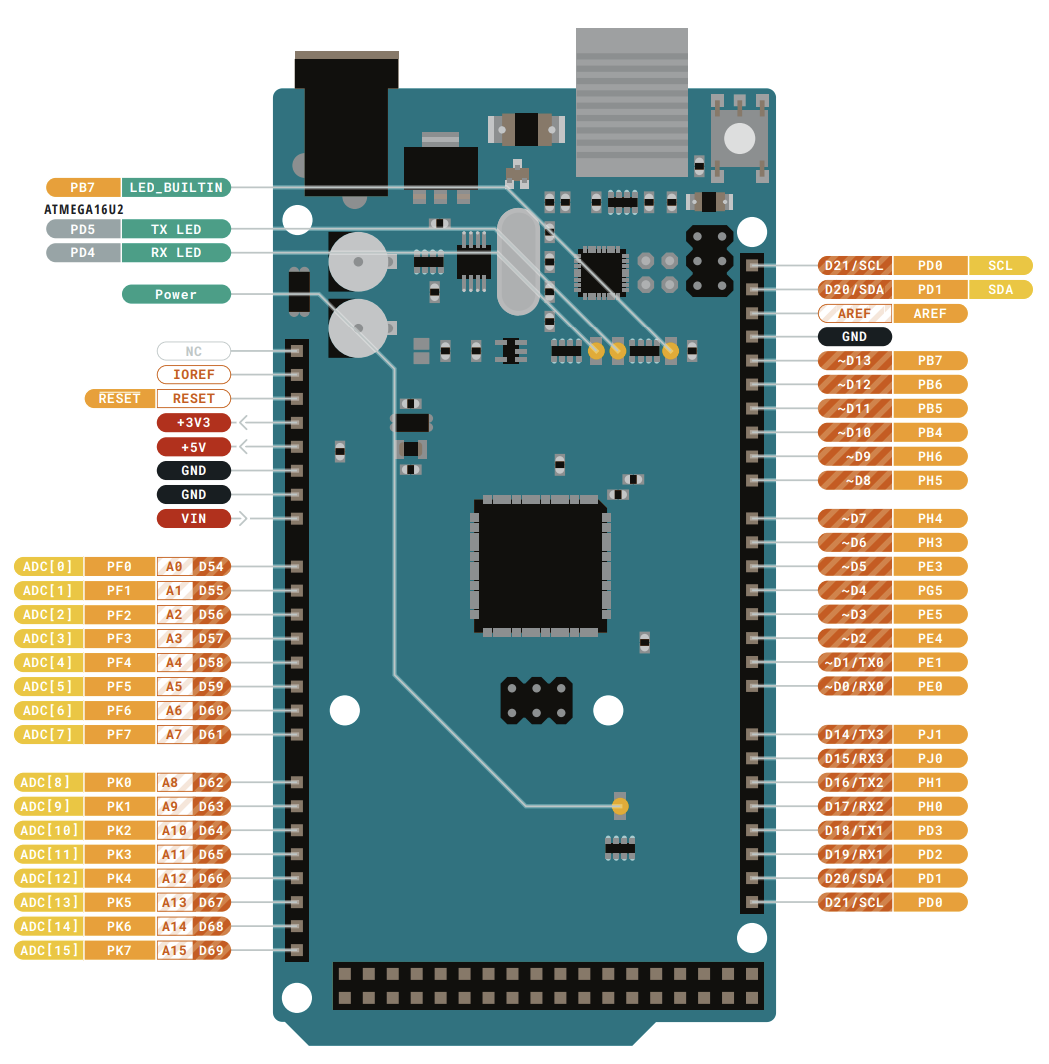
\includegraphics[width=1\textwidth]{imagenes/pinout_amega2560.png}
        \caption{Esquema de pines de la Arduino Mega 2560. Extraído de: [26]}
    \end{figure}
 

\section{Elección de periféricos}
 
Si bien no es una parte tan importante de la selección de componentes, escoger un buen periférico puede facilitar las labores de montaje y programación. No todos los periféricos pueden cuadrar en este proyecto, pues existen restricciones de precio y tamaño, por lo que se tiene que tener en cuenta estos parámetros a la hora de escoger. 



 \subsection*{Motor}

 En el caso de los motores, existen tres tipos principales: 

 \begin{enumerate}
  \item Motores DC: Son los más utilizados, aunque pueden requerir de un módulo de control o un puerto PWM para poder ser manejados con eficiencia.
  \item Motores paso a paso: Giran mediante pasos, siendo 1.8º y 3.75º las medidas más usuales. Requieren de un módulo para controlar su manejo.
  \item Servomotores: Son motores que únicamente pueden dar un giro de 180º, pero proporcionan un control total del giro.
 \end{enumerate}

 En este caso, la elección ha sido clara, los motores DC cumplen con todo lo necesario y además existen multitud de modelos. 
 Se ha escogido un motor básico, con eje para conectarse a la rueda, y se comprarán dos unidades para las dos ruedas delanteras del vehículo. 

 \subsubsection*{Placa de control de motor}

 Entre las dos alternativas más utilizadas, el driver L298H, con una capacidad para dos motores DC, y el escudo L293D, de la empresa MH Electronics, se ha escogido este último, debido a los cuatro puertos para motores DC. 

 \begin{figure}[H]
  \centering
  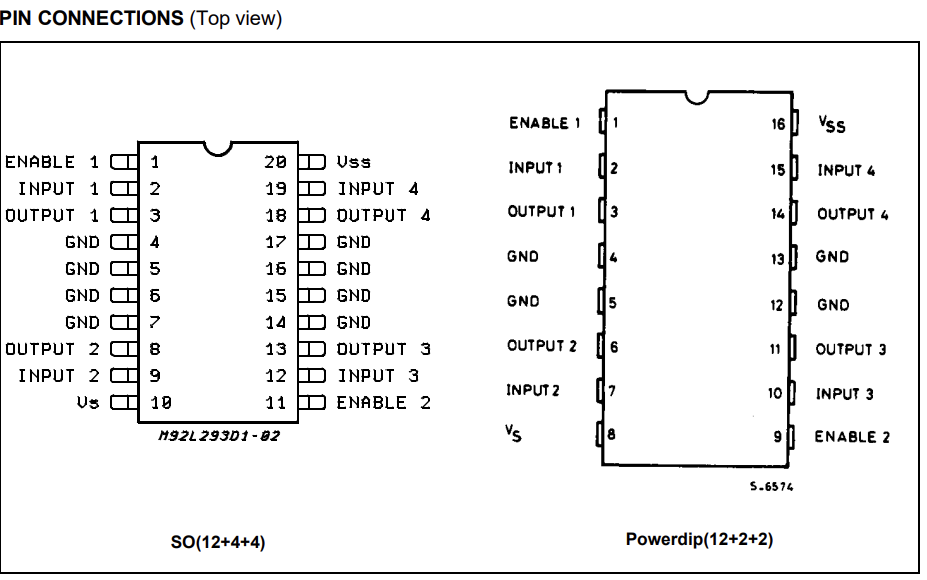
\includegraphics[width=1\textwidth]{imagenes/pinout_L293D.png}
  \caption{Esquema de pines del Shield L293D. Extraído de: [27]}
\end{figure}

 \subsection*{Sensores de temperatura}

 Respecto a los sensores de temperatura, se ha escogido el sensor DHT11. Aunque otras opciones tienen mejor tasa de muestreo, este sensor cubre las necesidades del proyecto, es muy barato, y ofrece una mayor documentación debido a su popularidad. 

 Se comprarán dos, uno para la temperatura del motor y otro para la batería.

 \subsection*{Sensor de voltaje}

[pend]

 \subsection*{Batería}
[pend]

\section{Componentes en situaciones reales}

Si bien estos componentes cumplen las necesidades del proyecto, nunca serían útiles en un entorno real. Esta ECU es una abstracción de una ECU real, en la que tendríamos que tener en cuenta muchos más factores tales como la temperatura, mayor fiabilidad en los sistemas, así como el resto de requerimientos que tendría un vehículo real. Además, los componentes que se utilizarían en un entorno real rondan los miles de euros, por lo que no es posible realizar un proyecto realista. 